\subsection{Definiciones}

\begin{frame}
  \frametitle{Aristas livianas y pesadas}

  Consideramos un árbol de \(N\) nodos.

  \vspace{0.75em}

  \begin{itemize}
    \item Por cada nodo con hijos, designamos como \textbf{hijo pesado} a aquel cuyo subárbol tiene la máxima cantidad de nodos (si hay más de uno, elegimos uno arbitrariamente).
    \item A las aristas que conectan nodos con su hijo pesado las llamamos \textbf{pesadas}.
    \item Si una arista no es pesada, la llamamos \textbf{liviana}.
    \item Terminología: a los caminos maximales formados enteramente por aristas pesadas los llamamos \textbf{caminos pesados}.
  \end{itemize}
\end{frame}

\begin{frame}
  \centering
  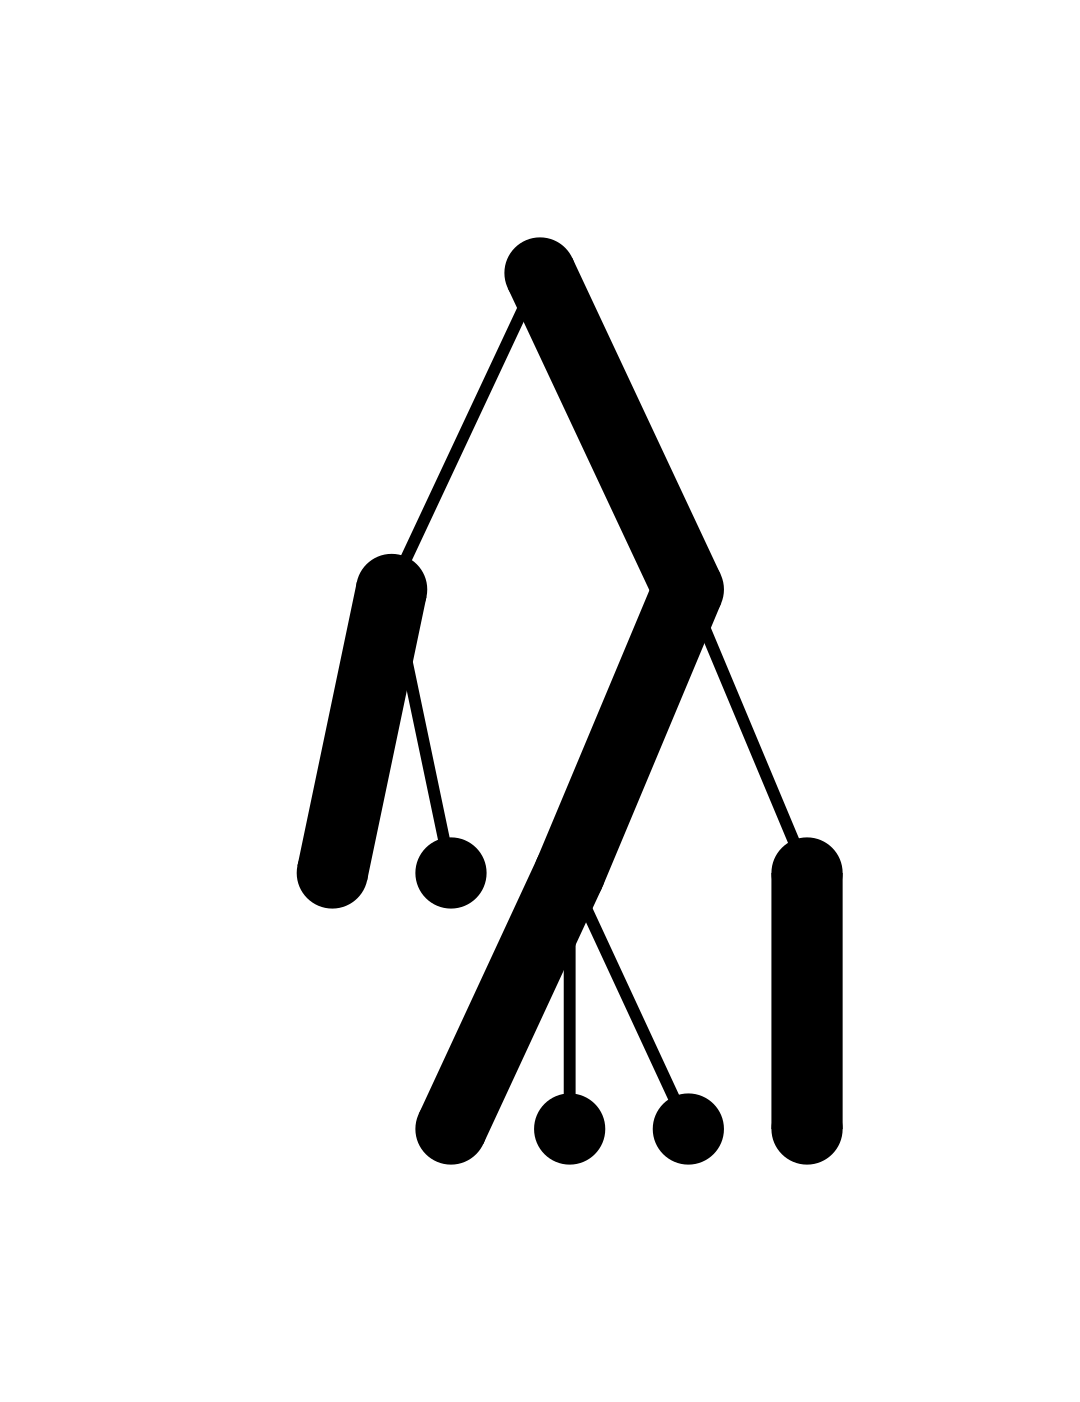
\includegraphics[height=0.85\textheight,keepaspectratio]{fotos/heavy.png}
\end{frame}

\begin{frame}
  \frametitle{Aristas livianas y pesadas: observaciones}

  \begin{block}{Observación clave}
    En un camino nodo--raíz puede haber a lo sumo \(\log_2 N\) aristas livianas.
  \end{block}

  \begin{center}
    \fbox{\parbox{0.85\textwidth}{\centering\vspace{1.5cm}\textit{[Diagrama: camino a la raíz con $\le \log_2 N$ aristas livianas]}\vspace{1.5cm}}}
  \end{center}
\end{frame}

\begin{frame}
  \frametitle{Aristas livianas y pesadas: más observaciones}

  \begin{block}{Observación clave}
    Claim similar para cantidad de caminos pesados que se tocan.
  \end{block}

  \vspace{0.5em}

  Otra forma de verlo: dado un camino cualquiera, puede tocar a lo sumo \(2 \log_2 N\) aristas livianas. A su vez, cada vez que toca una arista liviana cambia de camino pesado, por lo que puede tocar a lo sumo \(2 \log_2 N + 1\) caminos pesados distintos.

  \vspace{0.5em}

  O sea, un camino cualquiera se puede descomponer en ``pocas'' partes, cada una perteneciente a un camino pesado distinto.
\end{frame}

\begin{frame}[fragile]
  \frametitle{Heavy-light decompose: código}

\begin{lstlisting}
int n;
vector<int> g[maxn];

int s[maxn]; // tamano del subarbol
int p[maxn]; // padre (-1 si no tiene)
int h[maxn]; // hijo pesado (-1 si no tiene)

// calculo padres y tamanos de los subarboles
void dfs(int u) {
    s[u] = 1;
    for (int v : g[u]) if (v != p[u]) {
        p[v] = u;
        dfs(v);
        s[u] += s[v];
    }
}

void decompose(int root) {
    p[root] = -1;
    dfs(root);

    forn(u, n) {
        h[u] = -1;
        for (int v : g[u]) if (v != p[u]) {
            if (h[v] == -1 || s[h[v]] < s[v]) {
                h[u] = v;
            }
        }
    }
}
\end{lstlisting}
\end{frame}
